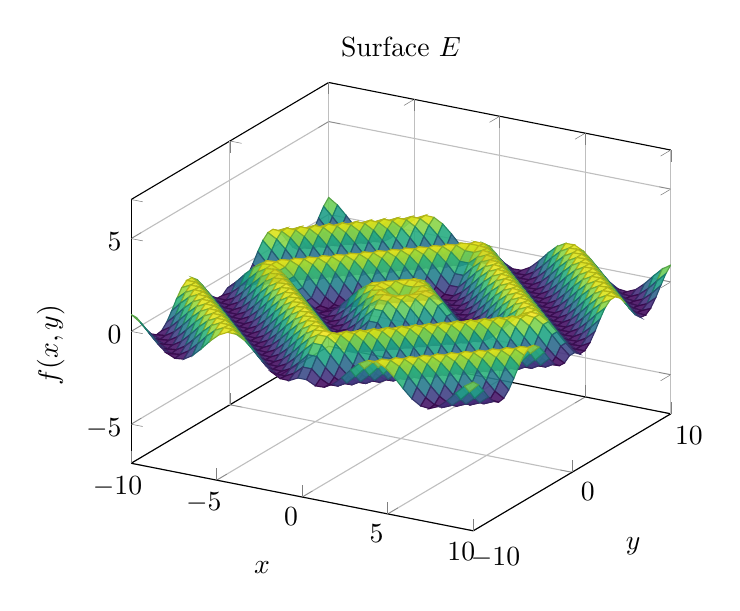
\begin{tikzpicture}[scale=1]
	\begin{axis}[
		title={Surface $E$},
		view={30}{20},
		colormap/viridis,
		xmin=-10, xmax=10,
		ymin=-10, ymax=10,
		zmin=-2, zmax=2,
		xlabel=$x$,
		ylabel=$y$,
		zlabel={$f(x,y)$},
		axis equal,
		grid=major
		]
		\addplot3[
		domain=-10:10,
		domain y=-10:10,
		samples=40,
		samples y=40,
		surf,
		fill opacity=0.9,
		] {sin((abs(x)+abs(y)) r)};
	\end{axis}
\end{tikzpicture}